%\documentclass[a4paper]{article}
%\usepackage[utf8]{inputenc}
\usepackage[spanish, es-tabla, es-noshorthands]{babel}
\usepackage[table,xcdraw,dvipsnames]{xcolor}
\usepackage[a4paper, footnotesep=1.25cm, headheight=1.25cm, top=2.54cm, left=2.54cm,
 bottom=2.54cm, right=2.54cm]{geometry}
%\geometry{showframe}
 \usepackage[normalem]{ulem}
 \useunder{\uline}{\ul}{}

%VERIFICAR EL HEAD Y EL FOOT EN
%https://ctan.dcc.uchile.cl/macros/latex/contrib/geometry/geometry.pdf

%Paquetes varios:
\usepackage{verbatimbox}

%\usepackage{wrapfig}			%Wrap figure in text
\usepackage[export]{adjustbox}	%Move images
\usepackage{changepage}			%Move tables
\usepackage{todonotes}

\usepackage{tikz}
\usepackage{amsmath}
\usepackage{amsfonts}
\usepackage{amssymb}
\usepackage{float}
\usepackage[graphicx]{realboxes}
\usepackage{caption}
\usepackage{subcaption}
\usepackage{multicol}
\usepackage{multirow}
\setlength{\doublerulesep}{\arrayrulewidth}
%\usepackage{booktabs}

\usepackage{array}
\newcolumntype{C}[1]{>{\centering\let\newline\\\arraybackslash\hspace{0pt}}m{#1}}
%\usepackage[american]{circuitikz}
\usetikzlibrary{calc}
\usepackage{fancyhdr}
\usepackage{units} 

\usepackage{colortbl}
%\usepackage{sectsty}
%\usepackage{unicode-math}

%FONTS (IMPORTANTE): Compilar en XeLaTex o LuaLaTeX
\usepackage{anyfontsize}	%Font size
\usepackage{fontspec}		%Font type
%Si sigue sin andar comentar \usepackage[utf8]{inputenc}
%https://ctan.dcc.uchile.cl/macros/unicodetex/latex/fontspec/fontspec.pdf
%https://www.overleaf.com/learn/latex/XeLaTeX

%Path para imagenes para trabajar en subarchivos
\graphicspath{{../Resumen/}{../Referencias/}{../Apendice/}{../Descripción de la Empresa/}{../Tareas del Alumno/}{../Conclusiones/}{../Herramientas Empleadas/}}

%Definiciones de nuevos comandos y colores
%COLORES:
\definecolor{AzulFoot}{rgb}{0.682,0.809,0.926}	%RGB	%{174,206,235}
\definecolor{AzulInfo}{rgb}{0.180,0.455,0.710}	%RGB	%{46,116,181}
\definecolor{AzulTable}{rgb}{0.302,0.507,0.871}	%RGB	%{68,114,196}
\definecolor{PName}{rgb}{0.353,0.353,0.353}		%RGB	%{90,90,90}
\definecolor{mygreen}{rgb}{28,172,0} % color values Red, Green, Blue
\definecolor{mylilas}{rgb}{170,55,241}

%Change Font Size

% #1 = size, #2 = text
\newcommand{\setparagraphsize}[2]{{\fontsize{#1}{6}\selectfont#2 \par}}		%Cambia el size de todo el parrafo
\newcommand{\setlinesize}[2]{{\fontsize{#1}{6}\selectfont#2}}				%Cambia el font de una oración

%IMAGE IN TABLE:			%Ejemplo: \includeintable{.3}{ImagenesFactibilidad/pend}
\renewcommand\fbox{\fcolorbox{white}{white}}
\setlength{\fboxrule}{0pt}	%padding thickness
\setlength{\fboxsep}{4pt}	%border thickness
\newcommand{\includeintable}[2]{	
	\fbox{
		\begin{minipage}{#1\textwidth}
        	\includegraphics[width=\linewidth]{#2}
    	\end{minipage}
	}
}

%LINK IN REF
\newcommand{\reflink}[1]{		%LINK
	\href{#1}{#1}
}

%NOTAS:
\newcommand{\note}[1]{		%RED BIG NOTE (TODO)
	\begin{center}
		\huge{ \textcolor{red}{#1} }
	\end{center}
}

\newcommand{\lnote}[1]{{\fontsize{14}{6}\selectfont\textcolor{green}{#1}}}	%Notas pequeñas

\newcommand{\observacion}[2]{  \ifnumequal{1}{#1}{ { \todo[inline,backgroundcolor=red!25,bordercolor=red!100]{\textbf{Observación: #2}} } }{  }  }

\newcommand{\red}[1]{\textcolor{red}{#1}}

\newcommand{\TBD}{\textcolor{red}{(TBD) }}
\newcommand{\tbd}{\textcolor{red}{(TBD) }}

\newcommand{\TBC}{\textcolor{red}{(TBC) }}
\newcommand{\tbc}{\textcolor{red}{(TBC) }}

\newcommand{\quotes}[1]{``#1''}
\newcommand{\q}[1]{``#1''}

\newcommand{\ip}{192.168.0.10:1880}
\newcommand{\ipadmin}{192.168.0.10:1880/admin}

% Comandos para agregar elementos en tablas de acronimos y definiciones
\newcommand{\addacronym}[2]{\textbf{#1} & \begin{tabular}[l]{@{}l@{}}#2\end{tabular} \\ \hline}

% tabItem
\newcommand{\tabitem}{~~\llap{\textbullet}~~}


\usepackage{hyperref}
\hypersetup{
    colorlinks=true,
    linkcolor=black,
    filecolor=magenta,      
    urlcolor=AzulInfo,
    citecolor=AzulInfo,    
}

%Configuración del header y del footer:
\usepackage{etoolbox}
\pagestyle{fancy}
\fancyhf{}
\rfoot{\thepage}
\renewcommand{\footrulewidth}{4pt}
\renewcommand{\headrulewidth}{0pt}
\patchcmd{\footrule}{\hrule}{\color{AzulFoot}\hrule}{}{}

%Código en el informe
%% IMPORTANTE:
% Verificar que esté \usepackage[dvipsnames]{xcolor}

%\usepackage{listingsutf8}
\usepackage{listings}

\renewcommand{\lstlistingname}{Código}

%LSTSET: Pone un recuadro y contador de linea en el codigo
\newcommand{\boxstyle}{
	\lstset{
		basicstyle=\sffamily\color{black},
		frame=single,
		numbers=left,
		numbersep=5pt,
		numberstyle=\color{gray},
		showspaces=false,
		showstringspaces=false
	}
}

\newcommand{\defaultstyle}{
	\lstset{
		basicstyle=\sffamily\color{white},
		frame=none,
		numbers=none,
		showspaces=true,
		showstringspaces=true
	}
}

\lstdefinelanguage{Kotlin}{
  captionpos=b,
  comment=[l]{//},
  commentstyle={\color{gray}\ttfamily},
  emph={filter, first, firstOrNull, forEach, lazy, map, mapNotNull, println},
  emphstyle={\color{OrangeRed}},
  identifierstyle=\color{black},
  keywords={!in, !is, abstract, actual, annotation, as, as?, break, by, catch, class, companion, const, constructor, continue, crossinline, data, delegate, do, dynamic, else, enum, expect, external, false, field, file, final, finally, for, fun, get, if, import, in, infix, init, inline, inner, interface, internal, is, lateinit, noinline, null, object, open, operator, out, override, package, param, private, property, protected, public, receiveris, reified, return, return@, sealed, set, setparam, super, suspend, tailrec, this, throw, true, try, typealias, typeof, val, var, vararg, when, where, while},
  keywordstyle={\color{NavyBlue}\bfseries},
  morecomment=[s]{/*}{*/},
  morestring=[b]",
  morestring=[s]{"""*}{*"""},
  ndkeywords={@Deprecated, @JvmField, @JvmName, @JvmOverloads, @JvmStatic, @JvmSynthetic, Array, Byte, Double, Float, Int, Integer, Iterable, Long, Runnable, Short, String, Any, Unit, Nothing},
  ndkeywordstyle={\color{BurntOrange}\bfseries},
  sensitive=true,
  stringstyle={\color{ForestGreen}\ttfamily},
}

\lstdefinelanguage{Swift}
{
  morekeywords={
    open,catch,@escaping,nil,throws,func,if,then,else,for,in,while,do,switch,case,default,where,break,continue,fallthrough,return,
    typealias,struct,class,enum,protocol,var,func,let,get,set,willSet,didSet,inout,init,deinit,extension,
    subscript,prefix,operator,infix,postfix,precedence,associativity,left,right,none,convenience,dynamic,
    final,lazy,mutating,nonmutating,optional,override,required,static,unowned,safe,weak,internal,
    private,public,is,as,self,unsafe,dynamicType,true,false,nil,Type,Protocol,
  },
  morecomment=[l]{//}, % l is for line comment
  morecomment=[s]{/*}{*/}, % s is for start and end delimiter
  morestring=[b]", % defines that strings are enclosed in double quotes
  breaklines=true,
  escapeinside={\%*}{*)},
  numbers=left,
  captionpos=b,
  breakatwhitespace=true,
  basicstyle=\linespread{1.0}\ttfamily, % https://tex.stackexchange.com/a/102728/129441
}

\definecolor{keyword}{HTML}{BA2CA3}
\definecolor{string}{HTML}{D12F1B}
\definecolor{comment}{HTML}{008400}

\newcommand{\swiftstyle}{
	\lstset{
  		language=Swift,
  		inputencoding=utf8x,
		extendedchars=\true,
	  	basicstyle=\ttfamily,
	  	showstringspaces=false, % lets spaces in strings appear as real spaces
  		columns=fixed,
  		keepspaces=true,
  		keywordstyle=\color{keyword},
  		stringstyle=\color{string},
  		commentstyle=\color{comment}
	}
}


%Como usarlo:

%\begin{lstlisting}[caption={Simple code listing.}, label={lst:example1}, language=Kotlin]
%// this is a simple code listing:
%println("hello kotlin from latex")
%\end{lstlisting}

%Si se corta en 2 páginas distintas:

%\vspace{1mm}
%\noindent{\begin{minipage}{\linewidth}
%\begin{lstlisting}[...]
%...
%\end{lstlisting}
%\end{minipage}}




\usepackage{titlesec}		%Para hacer las subsubsubsections

%Colores a los nombres de las secciones:
%\sectionfont{\color{AzulInfo}}  % sets color of sections
%\subsectionfont{\color{AzulInfo}}
%\subsubsectionfont{\color{AzulInfo}}

%PICTURES AND TABLE INDEX:
\newcommand{\Section}[1]{ \section{#1} 
	\phantomsection \setcounter{figure}{0} \setcounter{table}{0} \setcounter{lstlisting}{0}
		\renewcommand{\thetable}{\arabic{section}.\arabic{table}}
		\renewcommand{\thefigure}{\arabic{section}.\arabic{figure}}
		\renewcommand{\thelstlisting}{\arabic{section}.\arabic{lstlisting}}
}

\newcommand{\Subsection}[1]{ \subsection{#1}
	\phantomsection \setcounter{figure}{0} \setcounter{table}{0} \setcounter{lstlisting}{0}
		\renewcommand{\thetable}{\arabic{section}.\arabic{subsection}.\arabic{table}}
		\renewcommand{\thefigure}{\arabic{section}.\arabic{subsection}.\arabic{figure}}
		\renewcommand{\thelstlisting}{\arabic{section}.\arabic{subsection}.\arabic{lstlisting}}
}

\newcommand{\Subsubsection}[1]{ \subsubsection{#1} 
	\phantomsection \setcounter{figure}{0} \setcounter{table}{0}  \setcounter{lstlisting}{0}
		\renewcommand{\thetable}{\arabic{section}.\arabic{subsection}.\arabic{subsubsection}.\arabic{table}}
		\renewcommand{\thefigure}{\arabic{section}.\arabic{subsection}.\arabic{subsubsection}.\arabic{figure}}
		\renewcommand{\thelstlisting}{\arabic{section}.\arabic{subsection}.\arabic{subsubsection}.\arabic{lstlisting}}
}

%Definición de subsubsubsection:
\titleclass{\subsubsubsection}{straight}[\subsection]

\newcounter{subsubsubsection}[subsubsection]
\renewcommand\thesubsubsubsection{\thesubsubsection.\arabic{subsubsubsection}}

\titleformat{\subsubsubsection}
  {\normalfont\normalsize\bfseries\color{AzulInfo}}{\thesubsubsubsection}{1em}{}	%Color de subsubsubsection
\titlespacing*{\subsubsubsection}
{0pt}{3.25ex plus 1ex minus .2ex}{1.5ex plus .2ex}

\makeatletter
\renewcommand\paragraph{\@startsection{paragraph}{5}{\z@}%
  {3.25ex \@plus1ex \@minus.2ex}%
  {-1em}%
  {\normalfont\normalsize\bfseries}}
\renewcommand\subparagraph{\@startsection{subparagraph}{6}{\parindent}%
  {3.25ex \@plus1ex \@minus .2ex}%
  {-1em}%
  {\normalfont\normalsize\bfseries}}
\def\toclevel@subsubsubsection{4}
\def\toclevel@paragraph{5}
\def\toclevel@paragraph{6}
\def\l@subsubsubsection{\@dottedtocline{4}{7em}{4em}}
\def\l@paragraph{\@dottedtocline{5}{10em}{5em}}
\def\l@subparagraph{\@dottedtocline{6}{14em}{6em}}
\makeatother

\setcounter{secnumdepth}{4}
\setcounter{tocdepth}{4}

%Subsubsubsection:
\newcommand{\Subsubsubsection}[1]{ \subsubsubsection{#1} 
	\phantomsection \setcounter{figure}{0} \setcounter{table}{0} \renewcommand{\thetable}{\arabic{section}.\arabic{subsection}.\arabic{subsubsection}.\arabic{subsubsubsection}.\arabic{table}} \renewcommand{\thefigure}{\arabic{section}.\arabic{subsection}.\arabic{subsubsection}.\arabic{subsubsubsection}.\arabic{figure}}
}

%Tamaño, color e identación de sección, subsección, subsubsección y subsubsubsección:
%La identación de las subsecciones está tambien en Index-cfg.tex para el toc, lot y lot en el index
\titleformat{\section}[block]{\fontsize{16}{6}\selectfont\bfseries\color{AzulInfo}}{\thesection.}{1em}{} 
\titleformat{\subsection}[block]{\hspace{2.5em}\fontsize{13}{6}\selectfont\color{AzulInfo}}{\thesubsection}{1em}{}
\titleformat{\subsubsection}[block]{\hspace{3.5em}\fontsize{12}{6}\selectfont\color{AzulInfo}}{\thesubsubsection}{1em}{}
\titleformat{\subsubsubsection}[block]{\hspace{4em}\fontsize{11}{6}\selectfont\color{AzulInfo}}{\thesubsubsubsection}{1em}{}

%Pone las refrencias en el indice
\usepackage[numbib, nottoc, notlot, notlof]{tocbibind}

%Pone toc, lof y lot en colores y elijo el titulo de estos
\addto\captionsspanish{
	\renewcommand\contentsname{Contenidos}
	\renewcommand\listfigurename{Lista de Figuras}
	\renewcommand\listtablename{Lista de Tablas}
}

%Agrega TOC al indice
\renewcommand{\tableofcontents}{
	\stepcounter{section}
	\addcontentsline{toc}{section}{\protect\numberline{\thesection}\textbf{Contenidos}}
	\tableofcontents
}

%Agrega LOF al indice
\renewcommand{\listoffigures}{
	\stepcounter{section}
	\addcontentsline{toc}{section}{\protect\numberline{\thesection}\textbf{Lista de Figuras}}
	\listoffigures
}

%Agrega LOT al indice
\renewcommand{\listoftables}{
	\stepcounter{section}
	\addcontentsline{toc}{section}{\protect\numberline{\thesection}\textbf{Lista de Tablas}}
	\listoftables
}

%Indices: cambio la separación de los numeros para que entren tablas y fotos
\usepackage{tocloft}
\setlength{\cftfignumwidth}{1.35cm}  % change numwidth from figures in lof
\setlength{\cfttabnumwidth}{1.35cm}  % change numwidth from tables in lot
\renewcommand{\cfttoctitlefont}{\Large\bfseries\color{AzulInfo}}
\renewcommand{\cftloftitlefont}{\Large\bfseries\color{AzulInfo}}
\renewcommand{\cftlottitlefont}{\Large\bfseries\color{AzulInfo}}

%Coloca lineas punteadas a las seciones en el TOC
\renewcommand{\cftsecleader}{\cftdotfill{\cftdotsep}}

%Items con bullets y no cuadrados
\renewcommand{\labelitemi}{\textbullet }


%\begin{document}
En esta sección se analiza la confiabilidad de los elementos de \textit{hardware} y \textit{software}, exponiendo en cada caso los criterios utilizados. A su vez se separa la parte de \textit{hardware} observando cada parte de manera individual para luego obtener un resultado en conjunto.

\Subsection{Hardware}	
El estudio se lleva a cabo según la norma MIL-HDBK-217F, la cual estima la cantidad de fallas en unidad de tiempo para diferentes tipos de componentes electrónicos. Este estándar tiene en cuenta factores como las condiciones de uso, temperatura.

El primer paso consiste en realizar un gráfico de todos los módulos considerados críticos que garantizan las funcionalidades fundamentales del producto. Esto se presenta en la Figura (\ref{fig:criticos}).
\begin{figure}[H]
	\centering
	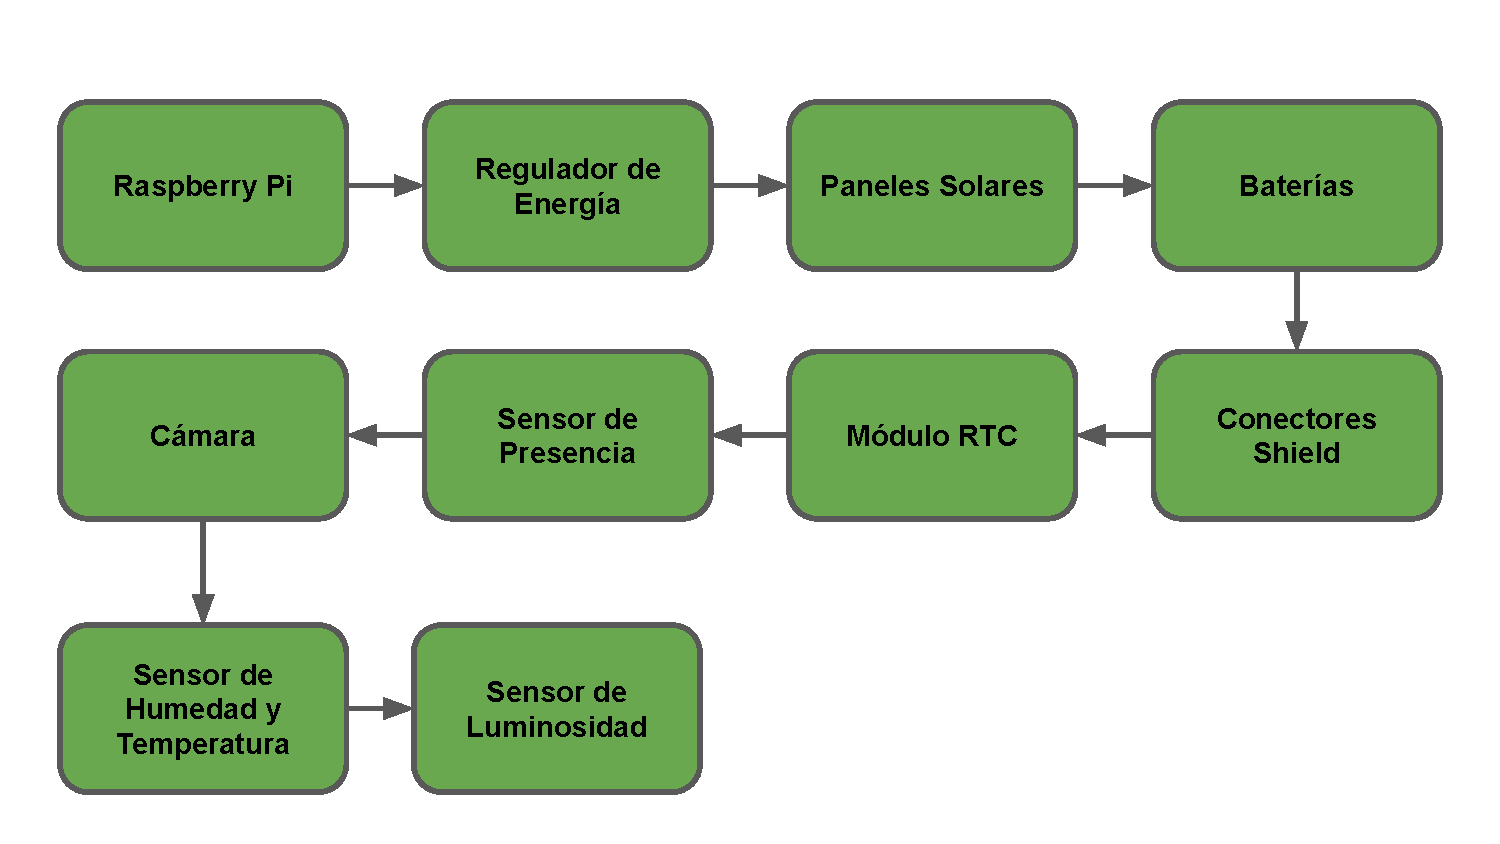
\includegraphics[width=0.9\linewidth,page=1]{ImagenesEstudios/ModulosCriticos}		
	\caption{Módulos críticos de funcionamiento.}
	\label{fig:criticos}
\end{figure}
Se calcula una estimación de la confiabilidad de cada módulo utilizando una estrategia \quotes{Top-Down}. Se encuentra la tasa de falla de cada submódulo mediante un proceso multiplicativo a la tasa de fallos base provista por las distintas cargas a las que son sometidos los componentes.
No se cuenta con redundancias, por lo que el valor de confiabilidad del módulo estará dado por la confiabilidad en serie de cada uno de sus componentes. Para todos los cálculos se considera una temperatura de 16$^{\circ}$C, la cual es la temperatura media de la zona d estudio en el periodo del mismo.
\begin{table}[H]
\centering
\begin{tabular}{|c|c|}
\hline
\textbf{Tipo de componente}   & \textbf{Cálculo de tasa de fallos $\left[\frac{\text{failures}}{10^6 \cdot \text{hour}}\right]$}                                                                               \\ \hline
\textbf{Resistencia}          & $\lambda_p \ = \ \lambda_b \ \cdot \  \pi_T \ \cdot \ \pi_P \ \cdot \ \pi_S \ \cdot \ \pi_Q \ \cdot \ \pi_E$                                                                   \\ \hline
\textbf{Capacitor}            & $\lambda_p \ = \ \lambda_b \ \cdot \  \pi_T \ \cdot \ \pi_C \ \cdot \ \pi_V \ \cdot \ \pi_{SR} \ \cdot \ \pi_Q \ \cdot \ \pi_E  $                                              \\ \hline
\textbf{IC DHT-22}            & $\lambda_p \ = \  (C_1 \ \cdot \ \pi_T \ + \ C_2 \ \cdot \ \pi_E ) \cdot \ \pi_Q \ \cdot \ \pi_L  $                                                                            \\ \hline
\textbf{IC BH1750}            & $\lambda_p \ = \lambda_{BD} \ \cdot \ \pi_{MFG} \ \cdot \ \pi_T \ \cdot \ \pi_{CD} \ + \ \lambda_{BP} \ \cdot \ \pi_E \ \cdot \ \pi_Q + \lambda_{EOS}$                         \\ \hline
\textbf{Shield}               & $\lambda_p \ = \ \lambda_b \ \cdot \  \pi_T \ \cdot \ \pi_K  \ \cdot \ \pi_Q \ \cdot \ \pi_E $                                                                                 \\ \hline
\textbf{Conexionado Sensores} & $\lambda_p \ = \ \lambda_b \ \cdot \  \pi_T \ \cdot \ \pi_K  \ \cdot \ \pi_Q \ \cdot \ \pi_E $                                                                                 \\ \hline
\textbf{IC DS1307}            & $\lambda_p \ = \lambda_{BD} \ \cdot \ \pi_{MFG} \ \cdot \ \pi_T \ \cdot \ \pi_{CD} \ + \ \lambda_{BP} \ \cdot \ \pi_E \ \cdot \ \pi_Q + \lambda_{EOS}$                         \\ \hline
\textbf{Diodo}                & $\lambda_p \ = \ \lambda_b \ \cdot \  \pi_T \ \cdot \ \pi_S  \ \cdot \ \pi_C \ \cdot \ \pi_Q \ \cdot \ \pi_E $                                                                 \\ \hline
\textbf{Regulador de Tensión} & $\lambda_p \ = \ \lambda_b \ \cdot \  \pi_T \ \cdot \ \pi_S  \ \cdot \ \pi_C \ \cdot \ \pi_Q \ \cdot \ \pi_E $                                                                 \\ \hline
\textbf{Transistor Mosfet}    & $\lambda_p \ = \ \lambda_b \ \cdot \  \pi_T \ \cdot \ \pi_A  \ \cdot \ \pi_R \ \cdot \ \pi_S \ \cdot \ \pi_Q \ \cdot \ \pi_E $                                                 \\ \hline
\textbf{VHSIC}                & \cellcolor[HTML]{FFFFFF}$\lambda_p \ = \lambda_{BD} \ \cdot \ \pi_{MFG} \ \cdot \ \pi_T \ \cdot \ \pi_{CD} \ + \ \lambda_{BP} \ \cdot \ \pi_E \ \cdot \ \pi_Q + \lambda_{EOS}$ \\ \hline
\textbf{Batería}              & \multicolumn{1}{c|}{Documentación}                                                                                                                                             \\ \hline
\textbf{Panel Solar}          & \multicolumn{1}{c|}{Documentación}                                                                                                                                             \\ \hline
\textbf{Cámara \rspi}          & \multicolumn{1}{c|}{Documentación}                                                                                                                                             \\ \hline
\textbf{Inductor}             & \multicolumn{1}{c|}{\cellcolor[HTML]{FFFFFF}$\lambda_p \ = \ \lambda_b \ \cdot \ \pi_T  \ \pi_Q \ \cdot \ \pi_E$}                                                              \\ \hline
\textbf{ESP8266}              & $\lambda_p \ = \  (C_1 \ \cdot \ \pi_T \ + \ C_2 \ \cdot \ \pi_E ) \cdot \ \pi_Q \ \cdot \ \pi_L  $                                                                            \\ \hline
\textbf{\rspi}                & \multicolumn{1}{c|}{Documentación}                                                                                                                                             \\ \hline
\end{tabular}
\caption{Ecuaciones para obtener la tasa de fallos de cada módulo acorde a MIL-HDBK-217F.}
\label{tasadefallos}
\end{table}

\Subsubsection{\rspi}
Para el módulo \rspi se utiliza la documentación de esta para obtener el valor de la tasa de fallos.
\begin{equation}
\lambda_p = 3 
\end{equation}
\Subsubsection{Regulador de Energía}
\begin{table}[H]
\centering
\begin{tabular}{|c|ccc|}
\hline
\textbf{Componente}          & \multicolumn{1}{c|}{\textbf{Cantidad}} & \multicolumn{1}{c|}{$\boldsymbol{\lambda_p}$}        & $\boldsymbol{\lambda_{Tot}}$ \\ \hline
\textbf{Capacitor}           & \multicolumn{1}{c|}{9}                 & \multicolumn{1}{c|}{\cellcolor[HTML]{FFFFFF}0.00356} & 0.03204                      \\ \hline
\textbf{Resistor}            & \multicolumn{1}{c|}{36}                & \multicolumn{1}{c|}{\cellcolor[HTML]{FFFFFF}0.00267} & 0.09612                      \\ \hline
\textbf{Diodo}               & \multicolumn{1}{c|}{7}                 & \multicolumn{1}{c|}{\cellcolor[HTML]{FFFFFF}0.0007}  & 0.0049                       \\ \hline
\textbf{Inductor}            & \multicolumn{1}{c|}{2}                 & \multicolumn{1}{c|}{0.06138}                         & 0.12276                      \\ \hline
\textbf{Transistores MOSFET} & \multicolumn{1}{c|}{13}                & \multicolumn{1}{c|}{0.1776}                          & 2.3088                       \\ \hline
\textbf{IC Step-Down}        & \multicolumn{1}{c|}{1}                 & \multicolumn{1}{c|}{1.106}                           & 1.106                        \\ \hline
\textbf{IC MPPT}             & \multicolumn{1}{c|}{1}                 & \multicolumn{1}{c|}{1.017}                           & 1.017                        \\ \hline
\textbf{IC Protocolo USB}    & \multicolumn{1}{c|}{1}                 & \multicolumn{1}{c|}{1.004}                           & 1.004                        \\ \hline
\textbf{Total}               & \multicolumn{1}{l}{}                   & \multicolumn{1}{l}{}                                 & \multicolumn{1}{r|}{5.69162} \\ \hline
\end{tabular}
\caption{Confiabilidad regulador de energía.}
\label{confReg}
\end{table}

\Subsubsection{Paneles Solares}
Para determinar a tasa de fallas de los paneles solares se utiliza la documentación de estos.
\begin{equation}
\lambda_p = 0.057 
\end{equation}

\Subsubsection{Baterías}
Para determinar a tasa de fallas de las baterías se utiliza la documentación.
\begin{equation}
\lambda_p = 0.005 
\end{equation}
\Subsubsection{Conector Shield}
\begin{table}[H]
\centering
\begin{tabular}{|c|ccc|}
\hline
\textbf{Componente}     & \multicolumn{1}{c|}{\textbf{Cantidad}} & \multicolumn{1}{c|}{$\boldsymbol{\lambda_p}$}        & $\boldsymbol{\lambda_{Tot}}$ \\ \hline
\textbf{Conectores PCB} & \multicolumn{1}{c|}{1}                 & \multicolumn{1}{c|}{\cellcolor[HTML]{FFFFFF}0.00182} & 0.00182                      \\ \hline
\textbf{Conector Molex} & \multicolumn{1}{c|}{1}                 & \multicolumn{1}{c|}{\cellcolor[HTML]{FFFFFF}0.00182} & 0.00182                      \\ \hline
\textbf{Total}          & \multicolumn{1}{l}{}                   & \multicolumn{1}{l}{\cellcolor[HTML]{FFFFFF}}         & \multicolumn{1}{r|}{0.00364} \\ \hline
\end{tabular}
\caption{Confiabilidad de la placa \textit{shield}.}
\label{confshield}
\end{table}

\Subsubsection{RTC}
% Please add the following required packages to your document preamble:
% \usepackage[table,xcdraw]{xcolor}
% If you use beamer only pass "xcolor=table" option, i.e. \documentclass[xcolor=table]{beamer}
\begin{table}[H]
\centering
\begin{tabular}{|c|ccc|}
\hline
\textbf{Componente} & \multicolumn{1}{c|}{\textbf{Cantidad}} & \multicolumn{1}{c|}{$\boldsymbol{\lambda_p}$}        & $\boldsymbol{\lambda_{Tot}}$ \\ \hline
\textbf{Capacitor}  & \multicolumn{1}{c|}{3}                 & \multicolumn{1}{c|}{\cellcolor[HTML]{FFFFFF}0.00356} & 0.01068                      \\ \hline
\textbf{Resistor}   & \multicolumn{1}{c|}{5}                 & \multicolumn{1}{c|}{\cellcolor[HTML]{FFFFFF}0.00267} & 0.01335                      \\ \hline
\textbf{Diodo}      & \multicolumn{1}{c|}{1}                 & \multicolumn{1}{c|}{\cellcolor[HTML]{FFFFFF}0.0007}  & 0.0007                       \\ \hline
\textbf{DS1307}     & \multicolumn{1}{c|}{1}                 & \multicolumn{1}{c|}{1.106}                           & 1.106                        \\ \hline
\textbf{Total}      & \multicolumn{1}{l}{}                   & \multicolumn{1}{l}{}                                 & \multicolumn{1}{r|}{1.13073} \\ \hline
\end{tabular}
\caption{Confiabilidad RTC.}
\label{confRTC}
\end{table}
\Subsubsection{Sensor de Presencia}
% Please add the following required packages to your document preamble:
% \usepackage[table,xcdraw]{xcolor}
% If you use beamer only pass "xcolor=table" option, i.e. \documentclass[xcolor=table]{beamer}
\begin{table}[H]
\centering
\begin{tabular}{|c|ccc|}
\hline
\textbf{Componente}     & \multicolumn{1}{c|}{\textbf{Cantidad}} & \multicolumn{1}{c|}{$\boldsymbol{\lambda_p}$}     & $\boldsymbol{\lambda_{Tot}}$ \\ \hline
\textbf{ESP32 WROOM S3} & \multicolumn{1}{c|}{1}                 & \multicolumn{1}{c|}{\cellcolor[HTML]{FFFFFF}1.08} & 1.08                         \\ \hline
\textbf{Total}          & \multicolumn{1}{l}{}                   & \multicolumn{1}{l}{\cellcolor[HTML]{FFFFFF}}      & \multicolumn{1}{r|}{1.08}    \\ \hline
\end{tabular}
\caption{Confiabilidad sensor de presencia.}
\label{tab:confpres}
\end{table}
\Subsubsection{Cámara \rspi}
Para determinar la tasa de fallas del módulo de cámara se recurre a la hoja de datos.
\begin{equation}
\lambda_p = 3.16
\end{equation}
\Subsubsection{Conector Sensores}
\begin{table}[H]
\centering
\begin{tabular}{|c|clc|}
\hline
\textbf{Componente}     & \multicolumn{1}{c|}{\textbf{Cantidad}} & \multicolumn{1}{c|}{$\boldsymbol{\lambda_p}$} & $\boldsymbol{\lambda_{Tot}}$  \\ \hline
\textbf{Conector Molex} & \multicolumn{1}{c|}{1}                 & \multicolumn{1}{r|}{0.00182}              & 0.00182                      \\ \hline
\textbf{Total}          & \multicolumn{1}{l}{}                   &                                           & \multicolumn{1}{r|}{0.00182} \\ \hline
\end{tabular}
\caption{Confiabilidad Conector Placa de Sensores}
\label{confsensores}
\end{table}
\Subsubsection{Sensor Humedad y Temperatura}
% Please add the following required packages to your document preamble:
% \usepackage[table,xcdraw]{xcolor}
% If you use beamer only pass "xcolor=table" option, i.e. \documentclass[xcolor=table]{beamer}
\begin{table}[H]
\centering
\begin{tabular}{|c|crc|}
\hline
\textbf{Componente}         & \multicolumn{1}{c|}{\textbf{Cantidad}} & \multicolumn{1}{c|}{$\boldsymbol{\lambda_p}$}        & $\boldsymbol{\lambda_{Tot}}$ \\ \hline
\textbf{Capacitor} & \multicolumn{1}{c|}{2}                 & \multicolumn{1}{r|}{0.00356}                         & 0.00712                      \\ \hline
\textbf{Resistor}  & \multicolumn{1}{c|}{1}                 & \multicolumn{1}{r|}{\cellcolor[HTML]{FFFFFF}0.00267} & 0.00267                      \\ \hline
\textbf{IC-DHT22}  & \multicolumn{1}{c|}{1}                 & \multicolumn{1}{r|}{3.036}                           & 3.036                        \\ \hline
\textbf{Total}     & \multicolumn{1}{l}{}                   & \multicolumn{1}{l}{}                                 & \multicolumn{1}{r|}{3.04579} \\ \hline
\end{tabular}
\caption{Confiabilidad Sensor de Temperatura y Humedad.}
\label{tab:conftemphum}
\end{table}
\Subsubsection{Sensor Luminosidad}

\begin{table}[H]
\centering
\begin{tabular}{|c|crc|}
\hline
\textbf{Componente}           & \multicolumn{1}{c|}{\textbf{Cantidad}} & \multicolumn{1}{c|}{$\boldsymbol{\lambda_p}$}        & $\boldsymbol{\lambda_{Tot}}$ \\ \hline
\textbf{Capacitor}            & \multicolumn{1}{c|}{4}                 & \multicolumn{1}{r|}{0.00356}                         & 0.01424                      \\ \hline
\textbf{Resistor}             & \multicolumn{1}{c|}{3}                 & \multicolumn{1}{r|}{\cellcolor[HTML]{FFFFFF}0.00267} & 0.00801                      \\ \hline
\textbf{Regulador de tensión} & \multicolumn{1}{c|}{1}                 & \multicolumn{1}{r|}{\cellcolor[HTML]{FFFFFF}0.00059} & 0.00059                      \\ \hline
\textbf{IC-BH1750}            & \multicolumn{1}{c|}{1}                 & \multicolumn{1}{r|}{1.106}                           & 1.106                        \\ \hline
\textbf{Total}                & \multicolumn{1}{l}{}                   & \multicolumn{1}{l}{}                                 & \multicolumn{1}{r|}{1.12884} \\ \hline
\end{tabular}
\caption{Confiabilidad Sensor de Luminosidad}
\label{tab:conflum}
\end{table}

\Subsubsection{Tasa de fallas total}
Utilizando los valores finales obtenidos en las anteriores tablas se calcula el $\lambda_{Total}$ de la siguiente manera:
\begin{equation}
\lambda_{Total} \ = \  \sum_{Modulos} \  \lambda_{Totn}  \  =  \ 18.8174 \  \frac{\text{fallas}}{10^6 \ \text{horas}}
\end{equation}
Luego asumiendo que $\lambda$ es constante y la función de confiabilidad definida como:
\begin{equation}
R(t) \ = \ e^{-\frac{\lambda_{Total}}{10^6}\ \cdot t}
\end{equation}
Con esto definido se obtiene el tiempo medio a la falla para todo el sistema:
\begin{equation}
MTTF \ = \ \int_0^\infty \ R(t)\ dt \ \approx \ 53142.19 \ \text{horas} \ \approx \ 6.066 \ \text{años}
\end{equation}
Además, se calcula valores para R(T) con un paso de 3 meses (Duración base del proyecto) hasta 3 años.
\begin{table}[H]
\centering
\begin{tabular}{|c|c|c|c|c|c|c|}
\hline
\textbf{Tiempo} & \textbf{3 Meses}                                                    & \textbf{6 Meses} & \textbf{9 Meses}                                                    & \textbf{1 Año}                                                      & \textbf{\begin{tabular}[c]{@{}c@{}}1 Año y\\ 3 Meses\end{tabular}}   & \textbf{\begin{tabular}[c]{@{}c@{}}1 Año y\\ 6 Meses\end{tabular}} \\ \hline
\textbf{$R(t)$} & 0.96                                                                & 0.922            & 0.885                                                               & 0.850                                                               & 0.816                                                                & 0.786                                                              \\ \hline
\textbf{Tiempo} & \textbf{\begin{tabular}[c]{@{}c@{}}1 Año y \\ 9 Meses\end{tabular}} & \textbf{2 Años}  & \textbf{\begin{tabular}[c]{@{}c@{}}2 Años y\\ 3 Meses\end{tabular}} & \textbf{\begin{tabular}[c]{@{}c@{}}2 Años y\\ 6 Meses\end{tabular}} & \textbf{\begin{tabular}[c]{@{}c@{}}2 Años y \\ 9 Meses\end{tabular}} & \textbf{3 Años}                                                    \\ \hline
\textbf{$R(t)$} & 0.752                                                               & 0.722            & 0.70 & 0.677                                                               & 0.647                                                                & 0.622                                                            \\ \hline
\end{tabular}
\caption{Probabilidad de confiabilidad con períodos de 3 meses.}
\label{probConf}
\end{table}

Teniendo en cuenta que el tiempo de vida del producto está estimado en 3 años y que la duración del estudio es de 3 meses. Que el tiempo medio a la falla sea de 6 años, resulta satisfactorio.
Finalmente cabe mencionar que luego de cada uso se recomienda una revisión técnica para asegurar un correcto funcionamiento de todos los módulos así aumentando la confiabilidad del sistema.
\Subsection{Software}
Para el estudio de confiabilidad de software se utilizó un modelo de estimación de tipo exponencial. Este modelo asume que todas las fallas que se presentan son independientes entre sí. Más específicamente se utilizará el modelo de Shooman, el cual normaliza las fallas por la cantidad de líneas de código $I_T$ sigue:
\begin{equation}
	R(t) = e^{-\lambda t}
\end{equation}
donde se toma
\begin{equation}
	\lambda = -k \left[ \epsilon_T - \epsilon(\zeta) \right]t
\end{equation}

Además, se define $\epsilon_T$ como la tasa de errores totales, $\epsilon(\zeta)$ la tasa de errores corregidos hasta un tiempo de corrección $\zeta$ y $k$ una constante del modelo de estimación.
\begin{table}[H]
\centering
\begin{tabular}{|c|c|c|c|c|c|c|c|c|}
\hline
\textbf{Semanas} & \boldmathcol{E_t}  		  & \boldmathcol{E_c}  			  & \boldmathcol{E_r}  			  & \textbf{H [hrs]} & \boldmathcol{\lambda_i}  & \boldmathcol{\frac{\lambda_i}{\lambda_{i-1}}}  & \boldmathcol{\hat{E}_{tot}}    & \boldmathcol{\hat{k}}    \\ \hline
1                & 20                         & 17                            & 3                             & 168              & 0.11905                  & -                                              & -                              & -                       \\ \hline
2                & 37                         & 33                            & 4                             & 336              & 0.05060                  & 0.42500                                        & 11.82609                       & 32.32474                \\ \hline
3                & 50                         & 43                            & 7                             & 504              & 0.02579                  & 0.50980                                        & 10.40000                       & 37.93184                \\ \hline
4                & 61                         & 52                            & 9                             & 672              & 0.01637                  & 0.63462                                        & 15.63158                       & 12.34174                \\ \hline
5                & 74                         & 65                            & 9                             & 840              & 0.01548                  & 0.94545                                        & 225.33333                      & 0.35769                 \\ \hline
6                & 89                         & 80                            & 9                             & 1008             & 0.01488                  & 0.96154                                        & 375.00000                      & 0.20329                 \\ \hline
7                & 105                        & 96                            & 9                             & 1176             & 0.01361                  & 0.91429                                        & 170.66667                      & 0.42079                 \\ \hline
8                & 115                        & 105                           & 10                            & 1344             & 0.00744                  & 0.54688                                        & 10.86207                       & 43.15476                \\ \hline
\end{tabular}
\caption{Fallas durante el periodo de test del \textit{software}.}
\label{tab:confsoft}
\end{table}

La Tabla (\ref{tab:confsoft}) presenta la cantidad acumulada de errores $E_t$, la cantidad acumulada de corregidos $E_c$, la cantidad acumulada resultante de los residuales $E_r$, las horas de test acumuladas \textbf{H [hrs]}, la tasa de fallos $\lambda$ y los parámetros invariables del modelo $\hat{E}_{tot}$ y $\hat{k}$ a lo largo del periodo de test. Estos son calculados mediante la formula:
\begin{equation}
	\hat{E}_{tot} = \frac{ \frac{\lambda_i}{\lambda_{i-1}} E_c(\tau_{i-1})-E_c(\tau_i)}{\frac{\lambda_i}{\lambda_{i-1}}-1}
\end{equation}
y
\begin{equation}
	\hat{k} = \lambda_i\frac{I_T}{\hat{E}_{tot}-E_c(\tau_i)}
\end{equation}

Finalmente, se adoptan los valores $\hat{E}_{tot} = 1$, $I_T = 5000$  y $\hat{k} = 43.15476$. Aproximando según
\begin{equation}
	\lambda = k\frac{E_r}{I_T}
\end{equation}
se obtiene $\lambda = 0.00863$ que, tomando el inverso de este valor se obtiene el $TMEF$, que resulta ser de $116 \ hs$. La tasa media entre fallos es pequeña, y se debe a dos errores a la hora de realizar el estudio de confiabilidad. Si bien este se realizó en una etapa tardía del desarrollo como postula la hipótesis del modelo, uno de los errores corregidos en la última etapa del \textit{testeo} redujo la frecuencia de aparición de errores subsiguientes significativamente. Además, la mayoría de los errores que surgieron eran de carácter visual y no impedían el correcto uso del programa. En la Tabla (\ref{tab:confsoft2}) se pueden observar valores de la función R(t).

\begin{table}[H]
\centering
\begin{tabular}{|c|c|c|c|c|c|}
\hline
\textbf{Tiempo} & \textbf{8 Horas} & \textbf{24 Horas} & \textbf{50 Horas} & \textbf{100 Horas} & \textbf{200 Horas} \\ \hline
$R(t)$          & 0.933            & 0.813             & 0.65              & 0.422              & 0.178              \\ \hline
\end{tabular}
\caption{Valores de la función probabilidad de confiabilidad de software.}
\label{probConf}
\end{table}

Otra cosa que cabe notar es que varios de los errores surgidos en la etapa de desarrollo eran de carácter acumulativo y tenían mayor probabilidad de aparición cuanto más tiempo se encuentre activo el software. Es por esto que se realiza cada ocho horas un reinicio del programa disminuyendo significativamente la tasa de apariencia de errores.

%\end{document}
